\documentclass[a4paper,norsk,12pt]{article}
\usepackage{amsmath,amssymb,amsthm}
\usepackage{graphicx}
\usepackage[norsk]{babel}
\usepackage[utf8]{inputenc}
\usepackage{float}
\usepackage{bm}
\usepackage{titling}
\usepackage{color}
\usepackage{verbatim}
\usepackage{listings}
\usepackage{subcaption}

\definecolor{mygreen}{RGB}{28,172,0} % color values Red, Green, Blue
\definecolor{mylilas}{RGB}{170,55,241}



\title{\vspace{-4.0cm} \textbf{Labøvelser - PRELAB, FYS1120-Elektromagnetisme}}
\author{Av: Laila Andersland}

\begin{document}
\maketitle


\lstset{language=Matlab,%
    %basicstyle=\color{red},
    breaklines=true,%
    morekeywords={matlab2tikz},
    keywordstyle=\color{blue},%
    morekeywords=[2]{1}, keywordstyle=[2]{\color{black}},
    identifierstyle=\color{black},%
    stringstyle=\color{mylilas},
    commentstyle=\color{mygreen},%
    showstringspaces=false,%without this there will be a symbol in the places where there is a space
    numbers=left,%
    numberstyle={\tiny \color{black}},% size of the numbers
    numbersep=9pt, % this defines how far the numbers are from the text
    emph=[1]{for,end,break},emphstyle=[1]\color{red}, %some words to emphasise
    %emph=[2]{word1,word2}, emphstyle=[2]{style},    
}

\section*{Del 1} 

\textbf{PRELAB-Oppgave 1} 

\noindent
\textit{Spenningen over en oppladet kondensator med $ C=1 \mu F$ som er koblet til inngangen på et voltmeter halveres på 20 sekunder. Hva er indre resistansen til voltmeteret?}

\vspace{3mm}

Potensialforskjellen:

$$U = U_0 e^{-t/ \tau}$$

Deler på $U_0$ og setter inn $\tau=RC$

$$ \dfrac{U}{U_0} = e^{-t/RC} $$


$$ ln (\dfrac{U}{U_0}) = -\dfrac{t}{RC} $$ 

Løser for \textit{R}:

\begin{equation}
R =  - \dfrac{t}{C} \cdot \dfrac{1}{ln ({U}/{U_0}) }
\end{equation}

Siden spenningen halveres fra iløpet av tidsforløpet:

$$ U = \dfrac{1}{2} U_0 $$

$$ \dfrac{U}{U_0} = \dfrac{\dfrac{1}{2} U_0}{U_0} $$

$$ \dfrac{U}{U_0} = \dfrac{1}{2} $$

Setter dette inn i (1):

$$ R =  - \dfrac{t}{C} \cdot \dfrac{1}{ln ({1}/{2}) } $$

Med $C = 1\mu F$ og tid $t=20s$ gir dette en resistansverdi, $ R = 2.88 \cdot 10^7 \Omega $

\newpage

\noindent
\textbf{PRELAB-Oppgave 2}

\noindent
\textit{Lag et MATLAB-script basert på.MATLAB-metodene polyfit og polyval som tilpasser en linje til et sett med datapunkter x,y og viser punktene og den tilpassede linjen på en figur.}

\lstinputlisting{interp.m}

\vspace{3mm}

Eksempel på bruk:

\begin{verbatim}
>> x=[500 700 1000 1500]

x =

         500         700        1000        1500

>> y = exp(x/500)

y =

    2.7183    4.0552    7.3891   20.0855
    
>> interp(x,y,3)  
\end{verbatim}

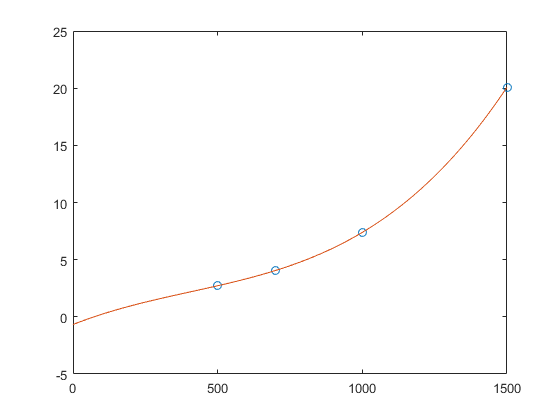
\includegraphics[width=70mm]{polyval.png}\\

\vspace{3mm}

\newpage

\noindent
\textbf{PRELAB-Oppgave 3}

\noindent
\textit{Finn et uttrykk for \textit{B} dersom vi dreier spolen med konstant vinkelhastighet $\omega$} og måler den maksimale verdien $\varepsilon_0$ for $\varepsilon(t)$. Hva er forholdet mellom $\omega$ og $t_2-t_1$

\vspace{3mm}

Sett fra siden, med B-felt i positiv x-retning:

\begin{figure}[H]
\centering
  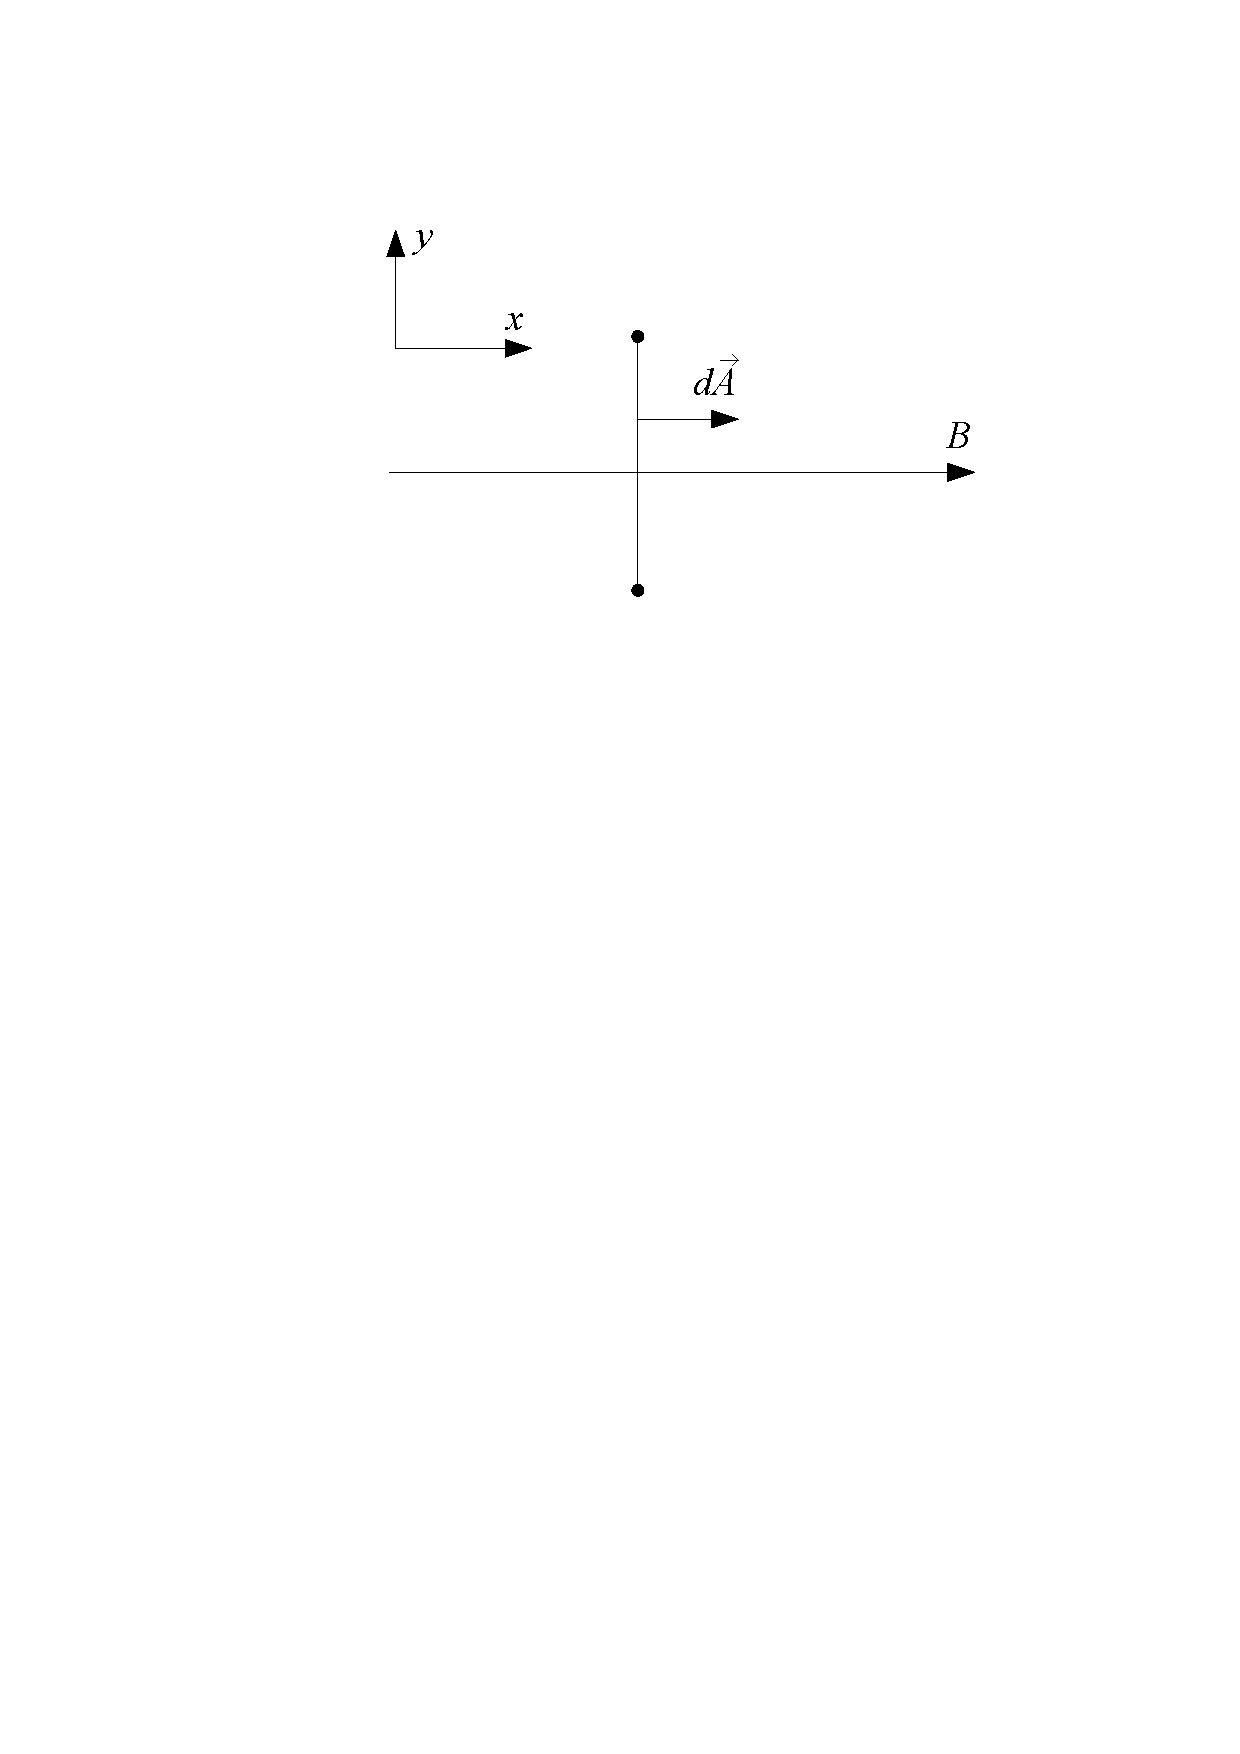
\includegraphics[width=\linewidth, trim={1cm 19cm 1cm 4cm},clip, width=0.8\textwidth,]{illuB.pdf}
  \caption{Illustrasjon av B-felt igjennom en spole.}
  \label{fig:plot11}
\end{figure}

Med N vindinger i spolen blir flukse:

$$ \Phi = N \int_A \vec{B} \cdot d \vec{A}  = N B A cos(\omega t) $$

Faradays lov gir:

$$ \varepsilon = - \dfrac{d \Phi}{dt} = N B A \omega sin(\omega t) $$

Siden maksimale spennignen,$ maks(\varepsilon) = \varepsilon_0 $, og $ maks(sin(\omega t)) = 1 $: 

$$ \varepsilon_0 = N B A  \omega $$

Løser for \textit{B}

\begin{equation}
B = \dfrac{\varepsilon_0}{N A \omega} 
\end{equation}

Vinkelhastigheten $\omega=\dfrac{rad}{s} $ gir en vinkel på $ 0 \leq \omega t \leq \pi $

Tiden vi bruker på å snu spolen $\pi$ grader er $t_2 - t_1$, og vi får da:

$$ \omega (t_2 - t_1) = \pi $$

Som gir forholdet:

$$ \omega = \dfrac{\pi}{(t_2 - t_1)} $$

Setter dette inn i (2) og får

$$ B = \dfrac{\varepsilon_0 (t_2 - t_1)}{N A \pi} $$ 

\end{document}